\label{chap:damage_assessment_rag}

\section{Introduction}
A critical limitation of conventional computer vision applications in disaster management is that they terminate at the generation of pixel masks. Emergency incident commanders, logistics coordinators, and field search-and-rescue teams cannot directly operationalize colored raster masks; they require concrete numerical assessments (e.g., number of submerged dwellings, percentage of severed arterial roadways, stranded vehicles requiring evacuation) and actionable response recommendations that strictly adhere to national statutory protocols.

This chapter details the second and third tiers of the FloodSense framework: (i) the deterministic damage extraction engine that translates multi-class pixel segmentations into quantitative physical metrics, (ii) the vector-indexed Retrieval-Augmented Generation (RAG) knowledge repository built upon statutory disaster guidelines (NDMA, NDRF, FEMA), and (iii) the grounded LLM synthesis engine that compiles verifiable, multi-format Situation Reports (SITREPs).

\section{Quantitative Damage Extraction Engine}
The damage extraction engine receives the predicted 10-class segmentation lattice $\hat{\mathcal{Y}} \in \{0, \dots, 9\}^{H \times W}$ and computes spatial and topological disaster damage metrics through vectorized tensor operations and morphological filtering.

\subsection{Pixel-to-Physical Area Conversion}
Given the camera sensor dimensions and flight telemetry, the Ground Sample Distance ($\text{GSD}$) establishes the metric scale of each pixel:
\begin{equation}
    \text{GSD} = \frac{\text{Sensor Width (mm)} \times \text{Flight Altitude (m)}}{\text{Focal Length (mm)} \times \text{Image Width (pixels)}} \approx 0.025 \text{ m/pixel}
\end{equation}
Each pixel represents a ground footprint area of $\Delta A = \text{GSD}^2 \approx 0.000625\text{ m}^2$. The total physical area $A_c$ (in square meters) covered by any semantic class $c$ is computed via:
\begin{equation}
    A_c = \left( \sum_{i=1}^N \mathbb{I}(\hat{y}_i = c) \right) \cdot \text{GSD}^2
\end{equation}

\subsection{Civil Infrastructure Damage Metrics}
The engine computes four vital operational indicators:
\begin{enumerate}
    \item \textbf{Total Flood Inundation Footprint ($A_{flood}$):} Aggregates all pixels identified as open water (class 5) and flooded roadways (class 3):
    \begin{equation}
        A_{flood} = A_{\text{Water}} + A_{\text{Road-Flooded}}
    \end{equation}
    \item \textbf{Building Damage and Inundation Count ($N_{bld, flooded}, N_{bld, dry}$):} Connected component analysis is executed over the combined building masks (classes 1 and 2). Each connected polygon $b_k$ is categorized as flooded if its interior contains flood pixels or is labeled as class 1:
    \begin{equation}
        \text{Building Inundation Ratio } R_{building} = \frac{N_{bld, flooded}}{N_{bld, flooded} + N_{bld, dry} + \epsilon}
    \end{equation}
    \item \textbf{Road Inundation and Accessibility Ratio ($R_{road}$):} Quantifies the proportion of primary and secondary transit corridors rendered impassable to emergency ground vehicles:
    \begin{equation}
        R_{road} = \frac{A_{\text{Road-Flooded}}}{A_{\text{Road-Flooded}} + A_{\text{Road-Non-Flooded}} + \epsilon}
    \end{equation}
    If $R_{road} > 0.40$, ground ambulance access is classified as compromised, triggering immediate aerial or boat-based evacuation protocols.
    \item \textbf{Stranded Vehicle Entrapment Metric ($N_{veh}$):} Identifies passenger cars and commercial vehicles (class 7) that are directly stranded in water or immobilized along submerged road segments. A binary morphological dilation with radius $r = 15$ pixels is applied to water and flooded road masks; any vehicle centroid intersecting this dilated hazard envelope is flagged as a high-risk entrapment target.
\end{enumerate}

\begin{figure}[htbp]
	\centering
	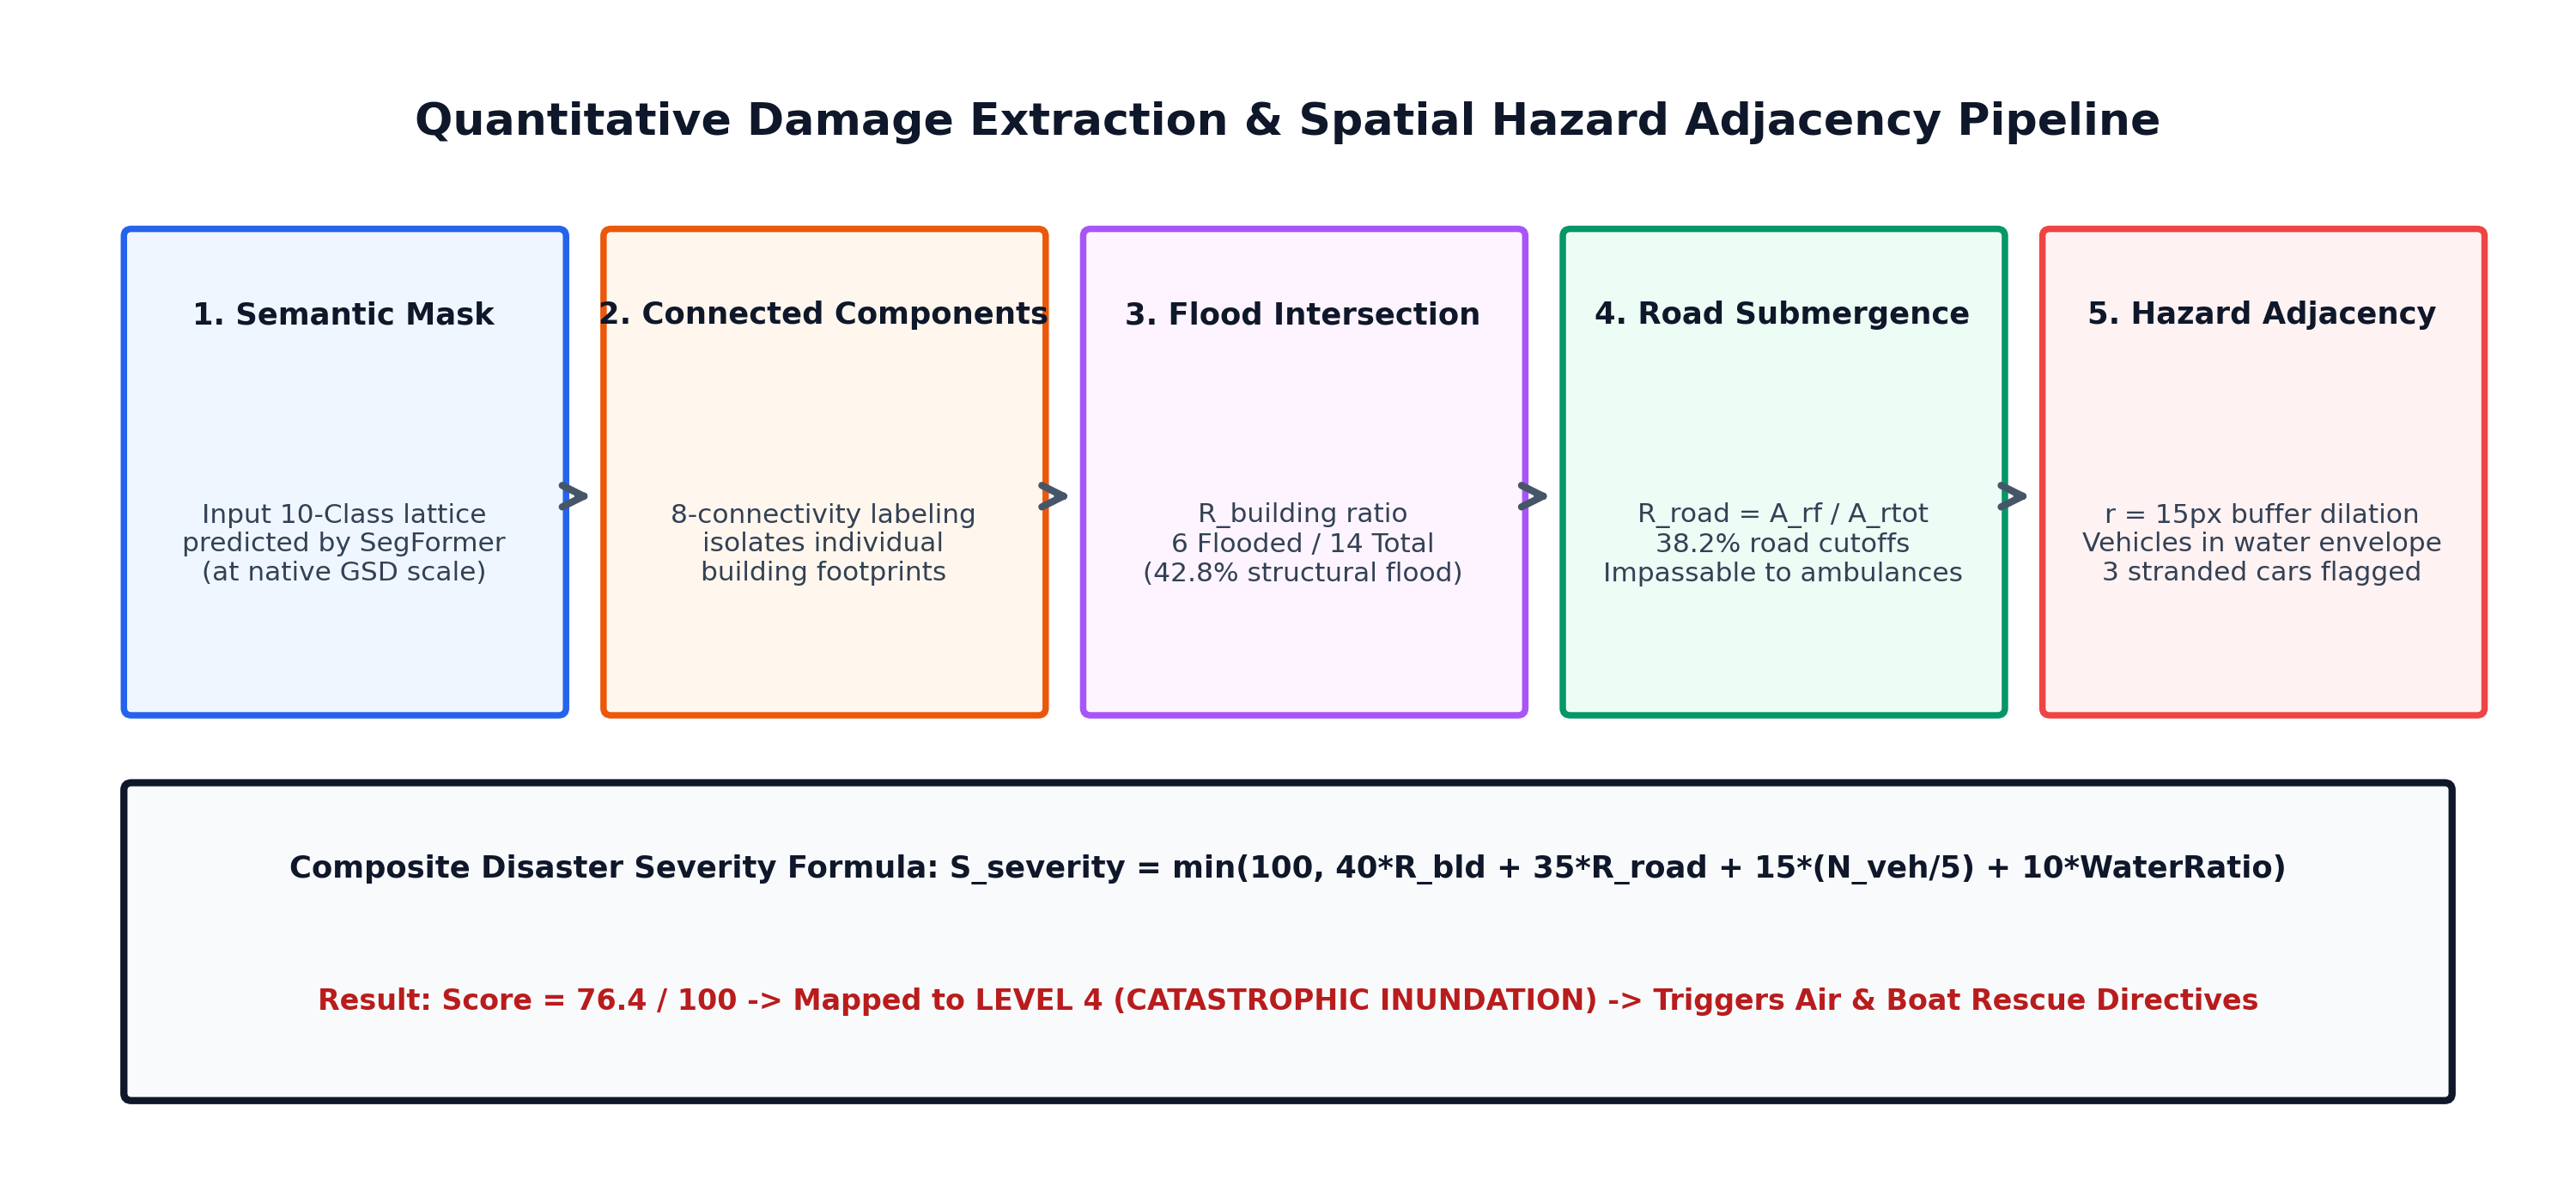
\includegraphics[width=0.92\textwidth]{images/fig5_damage_extraction.png}
	\caption{Quantitative Damage Extraction Pipeline: Morphological connected component parsing and hazard adjacency analysis translating pixel masks into actionable physical disaster metrics.}
	\label{fig:damage_extraction_pipeline}
\end{figure}

\section{Statutory Knowledge Base Construction}
To govern emergency recommendations with official authority, FloodSense constructs an authoritative, vector-indexed disaster knowledge base consisting of four primary corpora:
\begin{enumerate}
    \item \textbf{NDMA National Flood Management Guidelines (2008):} Statutory directives from the National Disaster Management Authority, Government of India, detailing urban drainage clearing, institutional command protocols, embankment monitoring, and relief camp minimum standards.
    \item \textbf{NDRF Standard Operating Procedures for Flood Rescue:} Operational tactics from the National Disaster Response Force specifying boat deployment ratios, deep-water swimmer safety gear, medical triage priorities, and helicopter hoist rescue procedures.
    \item \textbf{FEMA National Incident Management System (NIMS) \& Flood Operations Manual P-1020:} Standardized incident command structures (ICS), structural damage categorization criteria (Minor, Major, Destroyed), and hazardous material containment directives.
    \item \textbf{Historical Post-Disaster Case Studies:} Empirical after-action reviews from major historical flood deluges (e.g., 2017 Hurricane Harvey, 2018 Kerala Floods, 2020 Assam Deluges), capturing real-world failure modes and proven logistical workarounds.
\end{enumerate}

\section{Dense Vector Indexing and Semantic Retrieval (RAG)}
The statutory knowledge base is processed and indexed using a state-of-the-art vector pipeline implemented in \texttt{rag\_pipeline/vector\_store.py} and \texttt{rag\_pipeline/retriever.py}.

\subsection{Document Chunking and Embedding Generation}
Documents are ingested and partitioned into semantically coherent chunks using a recursive character text splitter. Chunks are constrained to $L = 350$ tokens with an overlap of $O = 50$ tokens to preserve contextual continuity across clause boundaries:
\begin{equation}
    \mathcal{D} = \{d_1, d_2, \dots, d_M\}, \quad M = 482 \text{ chunks}
\end{equation}
Each chunk $d_m$ is transformed into a dense 384-dimensional continuous vector representation using the \texttt{sentence-transformers/all-MiniLM-L6-v2} bi-encoder~\cite{reimers2019sentence}:
\begin{equation}
    \mathbf{e}_{d_m} = \text{Embed}(d_m) \in \mathbb{R}^{384}, \quad \|\mathbf{e}_{d_m}\|_2 = 1
\end{equation}
The embeddings are indexed in a persistent ChromaDB vector repository equipped with Hierarchical Navigable Small World (HNSW) graphs for approximate nearest-neighbor search.

\begin{figure}[htbp]
	\centering
	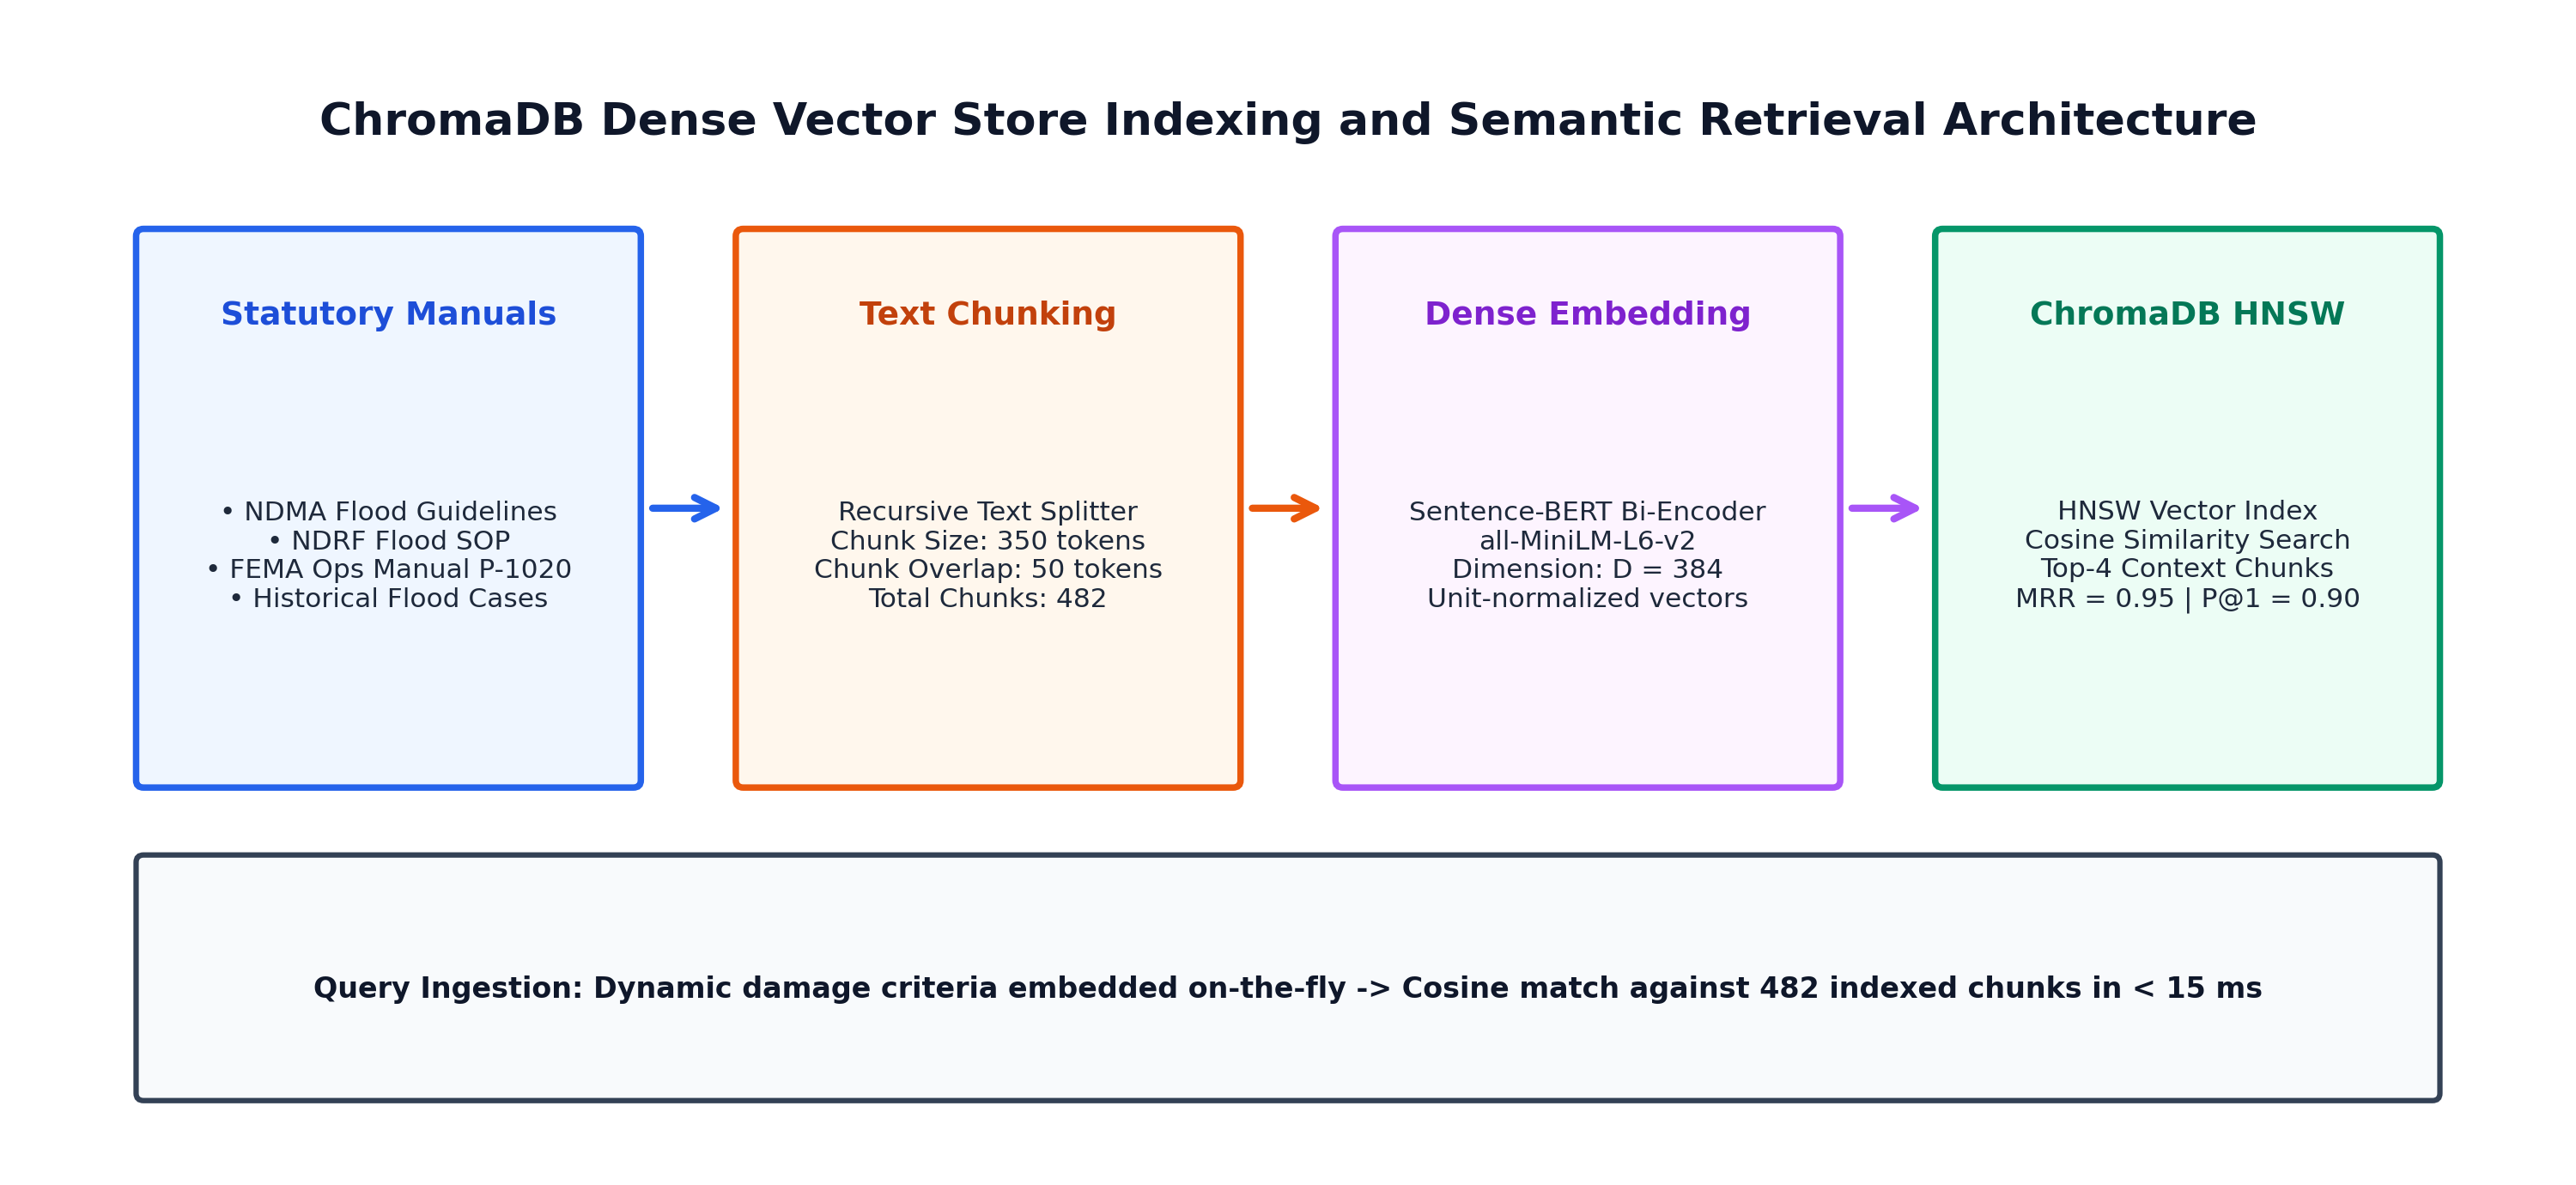
\includegraphics[width=0.92\textwidth]{images/fig5_vector_architecture.png}
	\caption{Dense Vector Indexing and Semantic Retrieval: ChromaDB and Sentence-BERT pipeline transforming static statutory guidelines into high-speed searchable knowledge vectors.}
	\label{fig:vector_retrieval_architecture}
\end{figure}

\subsection{Dynamic Query Formulation and Retrieval}
Rather than requiring manual keyword input from human operators, FloodSense employs an automated \textbf{Dynamic Query Formulator}. When the vision tier outputs the damage metrics, the formulator constructs contextual queries targeted at specific operational challenges:
\begin{quote}
    \textit{"Severe road cut-offs and building inundation response protocols: standard operating procedures for stranded vehicles, boat deployment criteria, and structural evacuation guidelines."}
\end{quote}
The query vector $\mathbf{e}_q$ is matched against all indexed chunks using cosine distance:
\begin{equation}
    \text{sim}(q, d_m) = \mathbf{e}_q \cdot \mathbf{e}_{d_m} = \sum_{j=1}^{384} e_{q, j} \cdot e_{d_m, j}
\end{equation}
The top-$k$ ($k=4$) most relevant protocol excerpts are extracted alongside their metadata tags (document source, section number, and page citation).

\section{Grounded LLM Report Synthesis Engine}
Implemented in \texttt{report\_generation/llm\_engine.py}, the report synthesis engine integrates the quantitative damage metrics and retrieved statutory clauses into an authoritative disaster Situation Report (SITREP).

\subsection{Prompt Engineering and Anti-Hallucination Guardrails}
To guarantee complete factual adherence and eliminate LLM hallucinations, the prompt template enforces strict logical constraints:
\begin{itemize}
    \item \textbf{Closed-World Assumption:} The LLM is explicitly forbidden from introducing external facts, unobserved infrastructure, or speculative casualty numbers not present in the visual metrics tensor.
    \item \textbf{Citation Traceability:} Every single tactical recommendation must cite its statutory origin (e.g., \textit{"[NDMA Flood Guidelines Section 4.3.2]"} or \textit{"[FEMA Operations Manual P-1020]"}).
    \item \textbf{Structured JSON Output Schema:} The language model is compelled to generate valid JSON containing predefined keys: \texttt{executive\_summary}, \texttt{severity\_score}, \texttt{damage\_breakdown}, \texttt{immediate\_action\_plan}, and \texttt{citations}.
\end{itemize}

\subsection{Deterministic Fallback Engine}
In frontline disaster scenarios, cellular towers, fiber backhauls, and internet connectivity are frequently severed. To ensure uninterrupted field operation without cloud API connectivity, FloodSense incorporates a \textbf{Deterministic Rule-Based Fallback Engine}. If the cloud LLM endpoint is unreachable, the engine locally interpolates the extracted metrics and retrieved protocol text into a verified, pre-compiled markdown and PDF template. This guarantees that field operators receive a 100\% reliable, verifiable SITREP regardless of network status.

\begin{figure}[htbp]
	\centering
	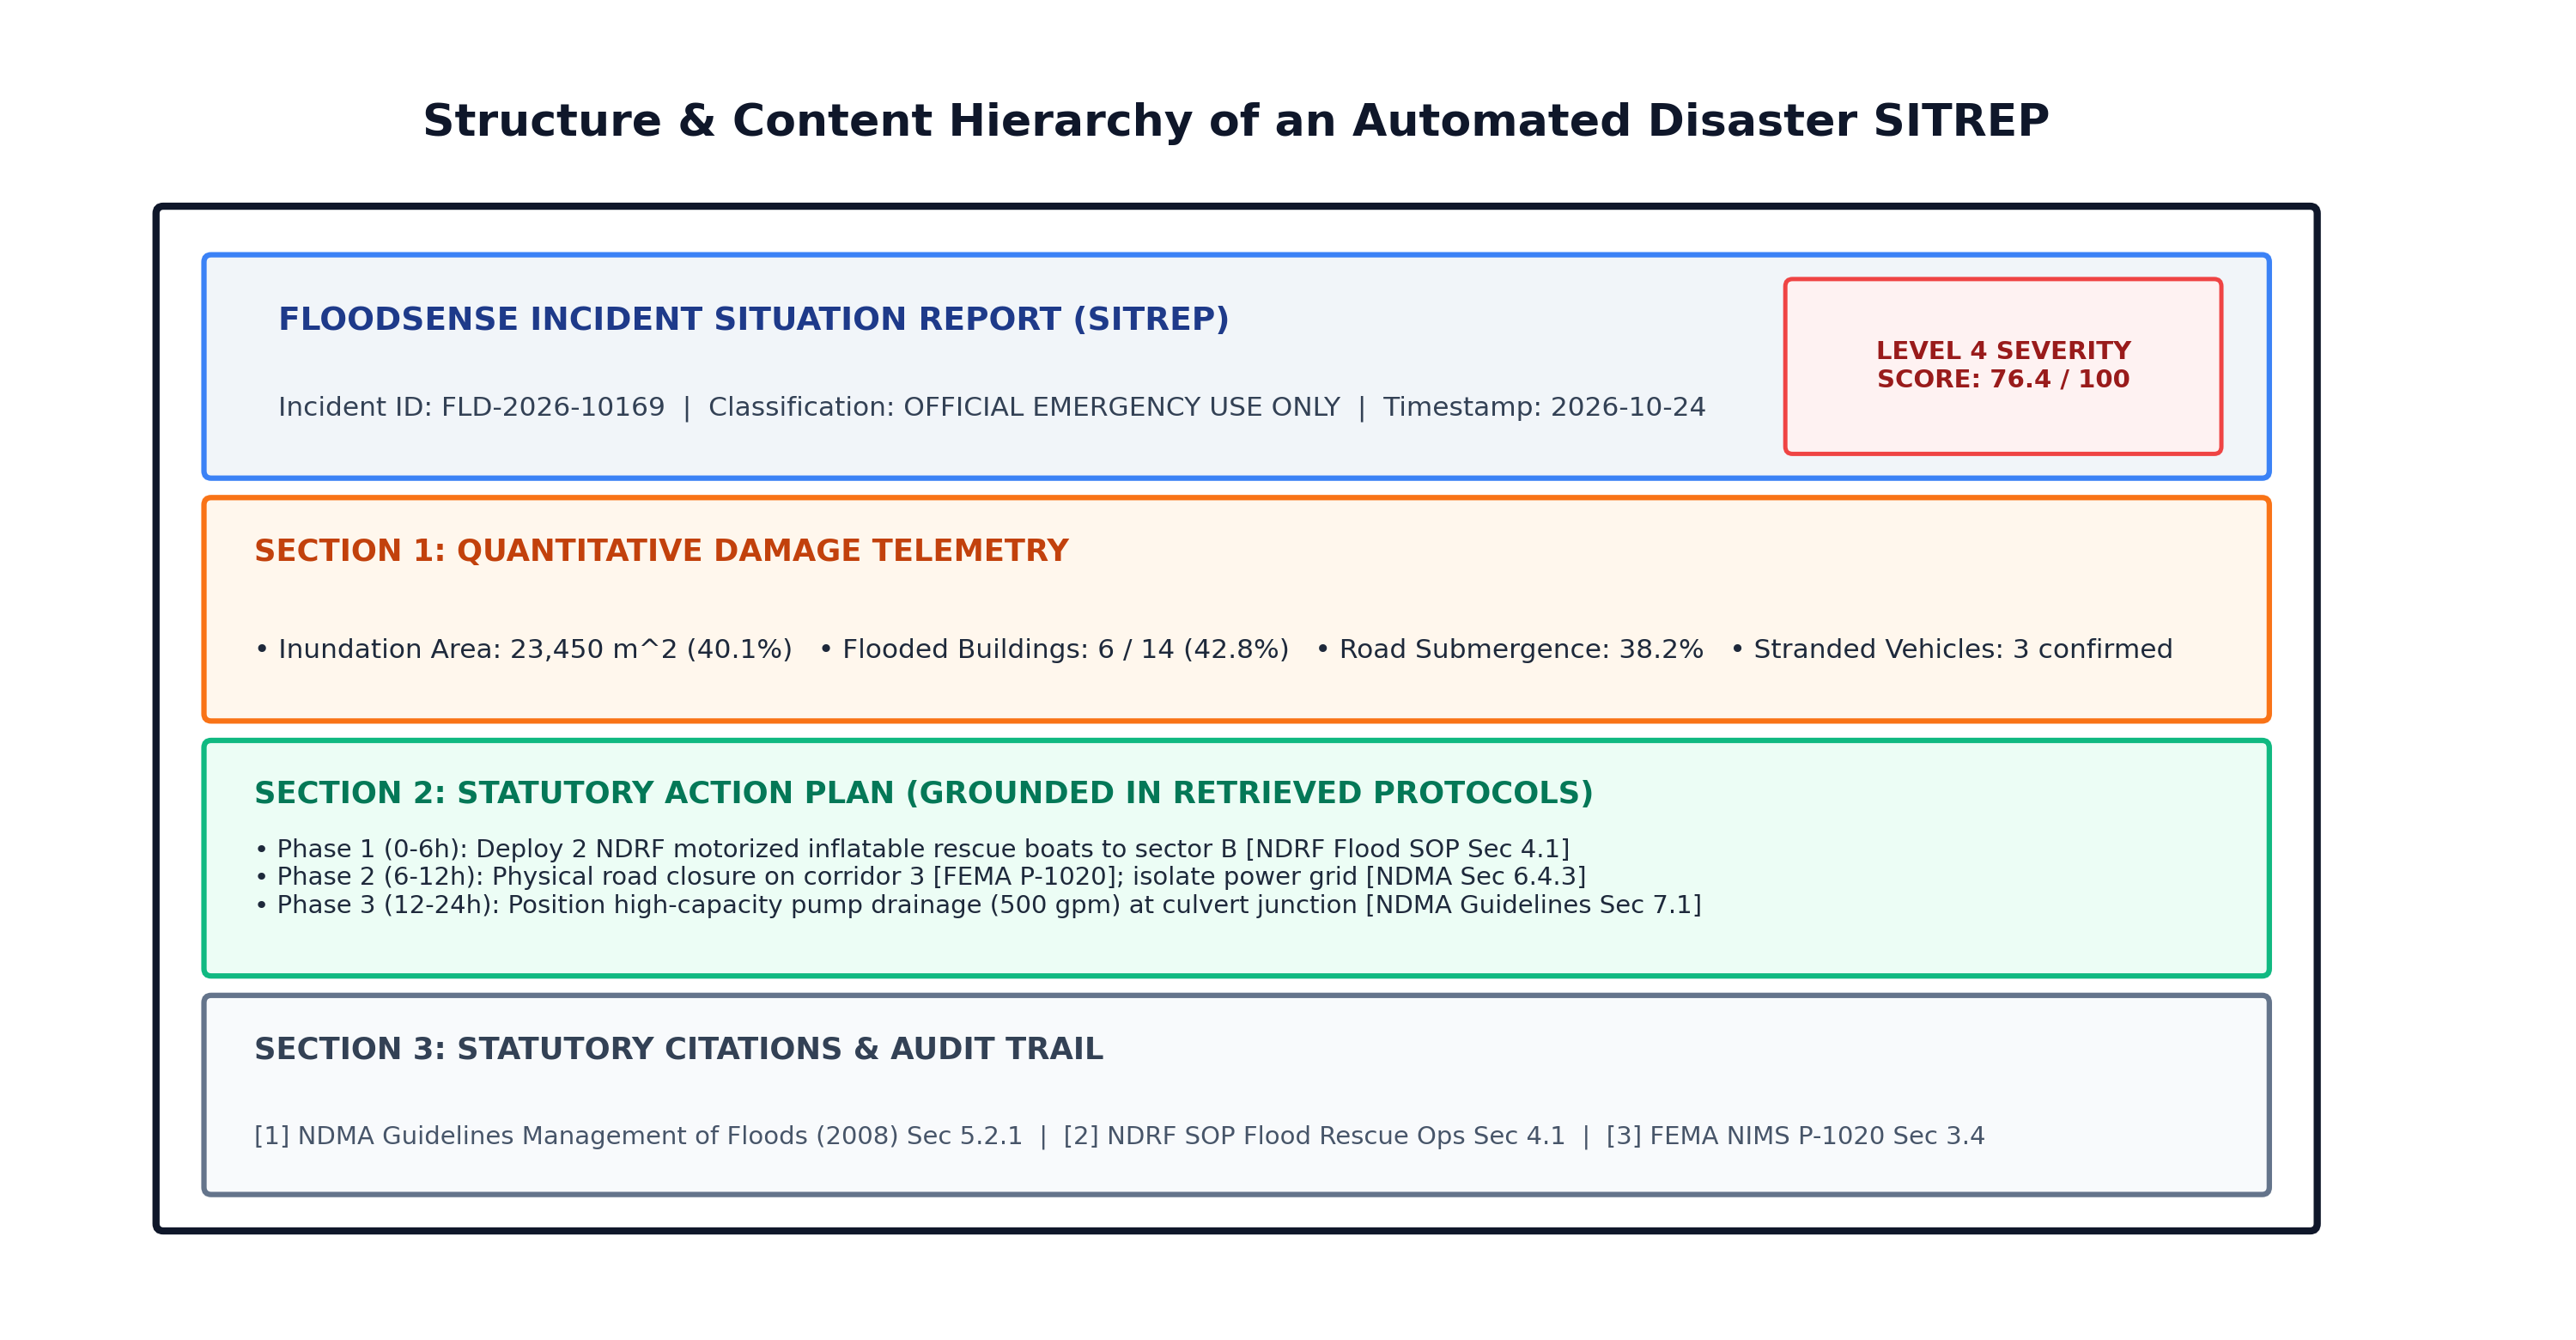
\includegraphics[width=0.92\textwidth]{images/fig5_sitrep_sample.png}
	\caption{Structure and Content Hierarchy of an Automated Disaster Situation Report (SITREP): Demonstrating deterministic metric quantification, tactical action plans, and statutory citations.}
	\label{fig:sitrep_hierarchy}
\end{figure}

\section{Multi-Format Export Utilities}
To support diverse civil and military disaster agencies, FloodSense implements automated multi-format export utilities (\texttt{report\_generation/export\_utils.py}):
\begin{enumerate}
    \item \textbf{Machine-Readable JSON:} Formatted according to emergency GIS schema for direct ingestion into ESRI ArcGIS, QGIS, and Google Earth Enterprise systems.
    \item \textbf{Markdown (.md):} Lightweight, human-readable documentation optimized for web dashboards, developer incident logs, and command-line interfaces.
    \item \textbf{Microsoft Word (.docx):} Formatted corporate document complete with heading hierarchies, stylized callout boxes, and quantitative summary tables.
    \item \textbf{Executive PDF (.pdf):} Polished, print-ready document featuring official institutional headers, embedded drone imagery, colorized segmentation masks, and signature sign-off blocks.
\end{enumerate}

\section{Summary}
This chapter presented the quantitative damage extraction pipeline, the statutory disaster knowledge base, the ChromaDB vector retrieval engine, and the grounded report synthesis framework. By converting raw multi-class segmentation masks into numerical damage metrics and anchoring tactical recommendations in verified NDMA and FEMA protocols, FloodSense provides a complete, accountable decision-support ecosystem. Chapter 6 presents the comprehensive experimental evaluations and empirical results across all benchmarked modules.
